\documentclass[10pt,aspectratio=169]{beamer}

% Theme selection
\usetheme{metropolis}
\metroset{progressbar=frametitle,block=fill,numbering=fraction}

% Packages
\usepackage{appendixnumberbeamer}
\usepackage{booktabs}
\usepackage{tabularx}
\usepackage{listings}
\usepackage{xcolor}
\usepackage{tikz}
\usepackage{tcolorbox}
\tcbuselibrary{skins,breakable}

% Color definitions (Shoestring Modern Palette)
\definecolor{ShoePrimary}{RGB}{24, 43, 73}      % Deep Navy
\definecolor{ShoeAccent}{RGB}{220, 80, 40}      % Burnt Orange / Coral
\definecolor{ShoeTeal}{RGB}{20, 140, 130}       % Electric Teal
\definecolor{ShoeGold}{RGB}{218, 165, 32}       % Amber Gold
\definecolor{ShoeBg}{RGB}{250, 250, 252}        % Soft canvas
\definecolor{ShoeCodeBg}{RGB}{240, 243, 246}    % Code background
\definecolor{ShoeGreen}{RGB}{34, 139, 34}       % Forest Green

\setbeamercolor{palette primary}{bg=ShoePrimary, fg=white}
\setbeamercolor{progress bar}{fg=ShoeAccent, bg=ShoePrimary!30}
\setbeamercolor{alerted text}{fg=ShoeAccent}
\setbeamercolor{frametitle}{bg=ShoePrimary, fg=white}
\setbeamercolor{block title}{bg=ShoePrimary, fg=white}
\setbeamercolor{block body}{bg=ShoePrimary!10, fg=black}
\setbeamercolor{block title alerted}{bg=ShoeAccent, fg=white}
\setbeamercolor{block body alerted}{bg=ShoeAccent!10, fg=black}
\setbeamercolor{block title example}{bg=ShoeTeal, fg=white}
\setbeamercolor{block body example}{bg=ShoeTeal!10, fg=black}

% Listings setup
\lstset{
    basicstyle=\ttfamily\scriptsize,
    backgroundcolor=\color{ShoeCodeBg},
    keywordstyle=\color{ShoeAccent}\bfseries,
    stringstyle=\color{ShoeTeal},
    commentstyle=\color{gray}\itshape,
    numberstyle=\tiny\color{gray},
    numbers=none,
    stepnumber=1,
    numbersep=8pt,
    showstringspaces=false,
    breaklines=true,
    frame=single,
    framerule=0.4pt,
    rulecolor=\color{gray!30},
    tabsize=2
}

% Title metadata
\title{AI on a Shoestring}
\subtitle{Champagne Intelligence on a Beer Budget: Local LLMs, Agents, RAG \& Colibr\`i}
\date{\today}
\author{Sudheer K. Mohammed}
\institute{BARC}
\titlegraphic{\hfill
\includegraphics[height=1.4cm,keepaspectratio]{images/shoestring_ai_logo.jpg}\hspace{0.5cm}
\includegraphics[height=1.4cm,keepaspectratio]{images/barc_logo.jpg}}

\begin{document}

% ----------------------------------------------------
% SLIDE 1: Title Slide
% ----------------------------------------------------
\maketitle

% ----------------------------------------------------
% SLIDE 2: The Shoestring Manifesto (Why Go Local?)
% ----------------------------------------------------
\begin{frame}{The Shoestring Manifesto}{Why Run AI Locally in 2026?}
    \begin{columns}[T]
        \begin{column}{0.55\textwidth}
            \textbf{The Pain of the Cloud Trap:}
            \begin{itemize}
                \item \alert{\$20/month fatigue}: 10 different subscriptions just to chat with bots.
                \item \textbf{Token Anxiety}: Every API call meters your wallet. One runaway loop = \$400 AWS invoice.
                \item \textbf{Privacy Roulette}: Uploading company trade secrets or diary entries to remote servers? No thanks.
                \item \textbf{Airplane Mode Zero}: Wi-Fi drops on the train? Your ``smart'' tools turn into doorstops.
            \end{itemize}
        \end{column}
        \begin{column}{0.42\textwidth}
            \begin{tcolorbox}[colback=ShoeAccent!10, colframe=ShoeAccent, title=\textbf{Shoestring Rule \#1}]
                \small
                ``Never pay a cloud giant for what an 8GB laptop and clever math can do while sitting on your couch unplugged.''
            \end{tcolorbox}
            \vspace{0.2cm}
            \begin{tcolorbox}[colback=ShoeTeal!10, colframe=ShoeTeal, title=\textbf{Our Goal Today}]
                \small
                From bare weights to full autonomous agents, RAG, and extreme MoE streaming---without spending a single dime.
            \end{tcolorbox}
        \end{column}
    \end{columns}
\end{frame}

% ----------------------------------------------------
% SLIDE 3: Narrow vs Broad AI: Sizing the Tool
% ----------------------------------------------------
\begin{frame}{Narrow vs. Broad AI}{Do You Need an AGI to Format a CSV?}
    \begin{columns}[T]
        \begin{column}{0.48\textwidth}
            \begin{block}{\textbf{Broad AI (Frontier Monsters)}}
                \begin{itemize}
                    \item 70B -- 1 Trillion+ parameters.
                    \item Writes Shakespearean sonnets about quantum physics while debugging Rust.
                    \item \textbf{Hardware cost}: Requires a small nuclear reactor and 8x A100/H100 clusters.
                    \item Overkill for 85\% of real-world productivity workflows!
                \end{itemize}
            \end{block}
        \end{column}
        \begin{column}{0.48\textwidth}
            \begin{exampleblock}{\textbf{Narrow / Small Language Models (SLMs)}}
                \begin{itemize}
                    \item 1B -- 8B parameters (Phi-3.5, Qwen-2.5, SmolLM, Llama-3.2).
                    \item Laser-focused on specific tasks: coding, summarization, tool invocation.
                    \item Often \textbf{outperforms} 70B behemoths on narrow domains with fine-tuning.
                    \item Runs comfortably in 4GB--8GB RAM!
                \end{itemize}
            \end{exampleblock}
        \end{column}
    \end{columns}
    \vspace{0.3cm}
    \centering
    \alert{\textbf{Key Insight:}} A nimble 3B model executing local scripts is $10\times$ faster and infinitely cheaper than waiting on a 400B cloud model.
\end{frame}

% ----------------------------------------------------
% SLIDE 4: Different Types of Models
% ----------------------------------------------------
\begin{frame}{The Model Zoo: Different Types for Different Jobs}
    \begin{table}
        \scriptsize
        \renewcommand{\arraystretch}{1.15}
        \begin{tabularx}{\textwidth}{@{}l l >{\raggedright\arraybackslash}X@{}}
            \toprule
            \textbf{Type} & \textbf{Examples} & \textbf{Superpower / Best Use} \\
            \midrule
            \textbf{Base Models} & Llama-3-8B-Base & Next-token completion only (don't chat with it!) \\
            \textbf{Instruct / Chat} & Qwen2.5-7B-Instruct & Follows commands, conversations, JSON output \\
            \textbf{Code-Specialized} & Qwen2.5-Coder, DeepSeek-Coder & Autocomplete, bug squashing, terminal scripts \\
            \textbf{Vision / Multimodal} & Llama-3.2-11B-Vision, Moondream & Extracts text from screenshots, UI inspection \\
            \textbf{Embedding Models} & BGE-small-en, Nomic-Embed & Vector search for RAG; tiny ($\sim$100MB), lightning fast \\
            \textbf{MoE (Mixture of Experts)} & Mixtral 8x7B, DeepSeek-V3 & Sparse activations; giant capacity, small compute \\
            \bottomrule
        \end{tabularx}
    \end{table}
    \vspace{0.15cm}
    \begin{tcolorbox}[colback=ShoePrimary!10, colframe=ShoePrimary, title=\textbf{Pro Tip}]
        \scriptsize
        Always check if a model suffix is \texttt{-Instruct} or \texttt{-Chat}. Chatting with a Base model feels like talking to someone who repeats your questions backwards!
    \end{tcolorbox}
\end{frame}

% ----------------------------------------------------
% SLIDE 5: What are AI Models & Formats?
% ----------------------------------------------------
\begin{frame}{Model Anatomy \& Weight Formats}
    \textbf{What is a model file really?} Just an enormous bundle of floating-point matrices ($\mathbf{W} \cdot \mathbf{x} + \mathbf{b}$) plus a tokenizer vocabulary.
    \vspace{0.2cm}
    \begin{columns}[T]
        \begin{column}{0.48\textwidth}
            \textbf{The Common Formats:}
            \begin{itemize}
                \item \textbf{PyTorch (\texttt{.bin} / \texttt{.pt})}:
                \begin{itemize}
                    \item Pickle-based, prone to arbitrary code execution security hazards. Deprecated!
                \end{itemize}
                \item \textbf{Safetensors (\texttt{.safetensors})}:
                \begin{itemize}
                    \item Developed by Hugging Face. Fast memory mapping (\texttt{mmap}), zero code execution. Cloud/Training standard.
                \end{itemize}
                \item \textbf{ONNX}:
                \begin{itemize}
                    \item Cross-platform execution, great for edge and browser runtimes.
                \end{itemize}
            \end{itemize}
        \end{column}
        \begin{column}{0.48\textwidth}
            \begin{tcolorbox}[colback=ShoeTeal!10, colframe=ShoeTeal, title=\textbf{The King of Local: GGUF}]
                \small
                \textbf{GGUF (GPT-Generated Unified Format):}
                \begin{itemize}
                    \item Created by Georgi Gerganov (\texttt{llama.cpp}).
                    \item Single self-contained file containing weights, metadata, tokenizer, and quantization tables.
                    \item Built for instantaneous memory mapping (\texttt{mmap}) into CPU RAM and GPU VRAM simultaneously!
                \end{itemize}
            \end{tcolorbox}
        \end{column}
    \end{columns}
\end{frame}

% ----------------------------------------------------
% SLIDE 6: Quantization: Squeezing Models
% ----------------------------------------------------
\begin{frame}{Quantization: Fitting Camels Through Needles}
    \begin{columns}[T]
        \begin{column}{0.50\textwidth}
            \textbf{Why Does Quantization Work?}
            \begin{itemize}\small
                \item Models train in 16-bit float (\texttt{FP16} = 2B/param).
                \item An 8B model in FP16 needs \textbf{16 GB VRAM}!
                \item Compresses continuous floats into discrete 8-bit, 4-bit, or 2-bit integer bins.
                \item Activations are noise-resilient: 4-bit preserves $\sim$98\% reasoning capability!
            \end{itemize}
            \vspace{0.15cm}
            \centering
            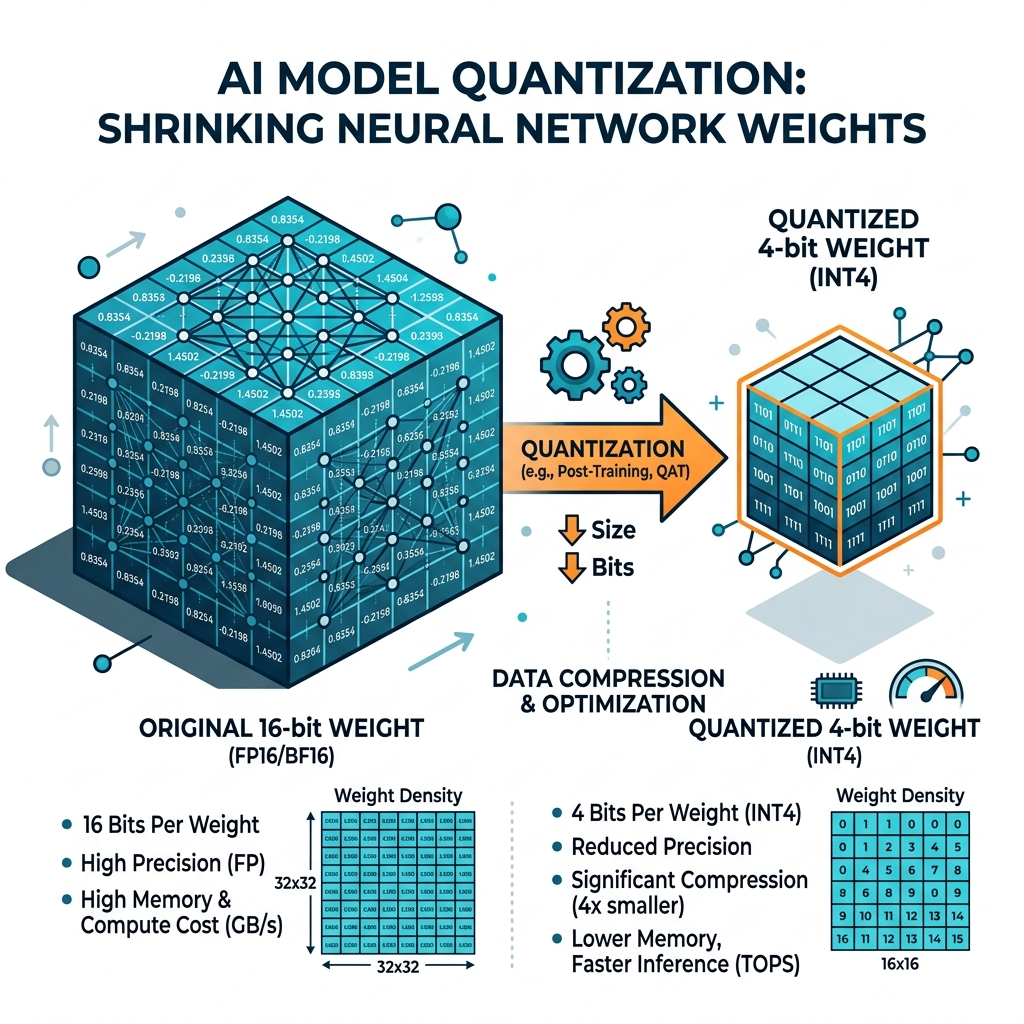
\includegraphics[height=2.3cm,keepaspectratio]{images/quantization.jpg}
        \end{column}
        \begin{column}{0.48\textwidth}
            \begin{table}
                \scriptsize
                \begin{tabular}{lll}
                    \toprule
                    \textbf{Quant} & \textbf{Size (8B)} & \textbf{Quality} \\
                    \midrule
                    FP16 & 16.0 GB & 100\% Baseline \\
                    Q8\_0 & 8.5 GB & Virtually lossless \\
                    \textbf{Q4\_K\_M} & \textbf{4.8 GB} & \textbf{Sweet Spot!} \\
                    Q3\_K\_S & 3.8 GB & Noticeable loss \\
                    Q2\_K & 2.9 GB & Hallucination fiesta \\
                    \bottomrule
                \end{tabular}
            \end{table}
            \vspace{0.15cm}
            \begin{tcolorbox}[colback=ShoeAccent!10, colframe=ShoeAccent, title=\textbf{Shoestring Rule \#2}]
                \scriptsize
                Always pick \textbf{Q4\_K\_M} (medium k-quant) first. It provides optimal quality-to-size balance on consumer PCs.
            \end{tcolorbox}
        \end{column}
    \end{columns}
\end{frame}

% ----------------------------------------------------
% SLIDE 7: Colibri Teaser #1
% ----------------------------------------------------
\begin{frame}{Shoestring Reality Check \& Colibr\`i Teaser}
    \begin{tcolorbox}[colback=ShoePrimary!10, colframe=ShoePrimary, title=\textbf{The Hardware Wall}]
        \large
        ``Okay, so an 8B model fits in 5GB RAM with Q4... \\
        What happens when you want to run a \textbf{744-Billion} frontier model on a \$700 laptop with 24GB of RAM?''
    \end{tcolorbox}
    \vspace{0.4cm}
    \begin{itemize}
        \item Normally: \alert{\textbf{Impossible}}. 744B in 4-bit needs $\sim$370 GB of VRAM. That's five \$30,000 Nvidia H100 servers!
        \item Standard reaction: ``Give up and pay OpenAI.''
        \item \textbf{Shoestring reaction}: ``Hold my coffee, let's look at the \textbf{Colibr\`i Project}.''
    \end{itemize}
    \vspace{0.3cm}
    \centering
    \textit{Keep this question in mind as we look at model architectures and runtimes...}
\end{frame}

% ----------------------------------------------------
% SLIDE 8: How to Run on PCs: The Local Trinity
% ----------------------------------------------------
\begin{frame}[fragile]{The Local Runtimes Trinity: llama.cpp, Ollama, LM Studio}
    \begin{columns}[T]
        \begin{column}{0.33\textwidth}
            \begin{block}{\textbf{1. llama.cpp}}
                \begin{itemize}
                    \item Pure C/C++ engine by Georgi Gerganov.
                    \item Zero dependencies, bare-metal CPU/GPU/Metal offloading.
                    \item Maximum speed and granular control.
                \end{itemize}
            \end{block}
        \end{column}
        \begin{column}{0.33\textwidth}
            \begin{exampleblock}{\textbf{2. Ollama}}
                \begin{itemize}
                    \item ``Docker for LLMs''.
                    \item One-line install, runs as background daemon.
                    \item Built-in OpenAI API compatible endpoint at \texttt{11434}.
                \end{itemize}
            \end{exampleblock}
        \end{column}
        \begin{column}{0.33\textwidth}
            \begin{alertblock}{\textbf{3. LM Studio}}
                \begin{itemize}
                    \item Beautiful desktop GUI for Mac, Windows, Linux.
                    \item 1-click download from Hugging Face.
                    \item Built-in chat, token metrics, local server toggle.
                \end{itemize}
            \end{alertblock}
        \end{column}
    \end{columns}
    \vspace{0.3cm}
    \begin{block}{Getting Started in 10 Seconds (Ollama)}
\begin{lstlisting}[language=bash]
# Pull and chat with a state-of-the-art 3B instruction model
curl -fsSL https://ollama.com/install.sh | sh
ollama run llama3.2:3b "Explain quantum physics like I'm five"
\end{lstlisting}
    \end{block}
\end{frame}

% ----------------------------------------------------
% SLIDE 9: Hugging Face Ecosystem
% ----------------------------------------------------
\begin{frame}{The Hugging Face Safari: Navigating the Model Jungle}
    \begin{columns}[T]
        \begin{column}{0.55\textwidth}
            \textbf{What is Hugging Face?}
            \begin{itemize}
                \item The GitHub + App Store of machine learning.
                \item Host for 1,000,000+ open-source models, datasets, and interactive Spaces.
            \end{itemize}
            \vspace{0.2cm}
            \textbf{How a Shoestring Hacker Uses It:}
            \begin{itemize}
                \item \textbf{Model Cards}: Check license (Apache 2.0 vs Llama community license vs non-commercial).
                \item \textbf{Quantization Legends}: Search for repositories by \texttt{bartowski} or \texttt{TheBloke}. They pre-quantize almost every hot release into GGUF!
                \item \textbf{Open LLM Leaderboard}: Filter by parameter count ($<8\text{B}$) to spot punching-above-their-weight SLMs.
            \end{itemize}
        \end{column}
        \begin{column}{0.42\textwidth}
            \begin{tcolorbox}[colback=ShoeGold!10, colframe=ShoeGold, title=\textbf{Search Anatomy}]
                \small
                \texttt{Qwen/Qwen2.5-7B-Instruct-GGUF}\\
                $\downarrow$\\
                \textbf{Creator}: Qwen team\\
                \textbf{Model}: Qwen2.5\\
                \textbf{Size}: 7B parameters\\
                \textbf{Tuning}: Instruct (ready for tasks)\\
                \textbf{Format}: GGUF (ready for local)
            \end{tcolorbox}
            \vspace{0.2cm}
            \alert{\textbf{Pro Tip:}} Never download blind raw safetensors unless you have 64GB VRAM and a weekend to convert them!
        \end{column}
    \end{columns}
\end{frame}

% ----------------------------------------------------
% SLIDE 10: Dense vs Mixture of Experts (MoE)
% ----------------------------------------------------
\begin{frame}{Dense Models vs. Mixture-of-Experts (MoE)}
    \begin{columns}[T]
        \begin{column}{0.48\textwidth}
            \begin{block}{\textbf{Dense Architectures}}
                \begin{itemize}
                    \item Every single weight is multiplied for \textbf{every single token}.
                    \item Example: Llama-3-8B fires all 8B parameters on every word.
                    \item Simple, predictable, but computationally expensive as size scales.
                \end{itemize}
            \end{block}
        \end{column}
        \begin{column}{0.48\textwidth}
            \begin{exampleblock}{\textbf{Mixture-of-Experts (MoE)}}
                \begin{itemize}
                    \item Decomposes feed-forward layers into $N$ specialized ``experts''.
                    \item A lightweight \textbf{router} selects top-$K$ experts per token (e.g., 2 out of 8).
                    \item Example: Mixtral 8x7B has 47B total params, but only computes 13B per token!
                \end{itemize}
            \end{exampleblock}
        \end{column}
    \end{columns}
    \vspace{0.4cm}
    \begin{tcolorbox}[colback=ShoeTeal!10, colframe=ShoeTeal, title=\textbf{The Shoestring Epiphany}]
        \small
        If only 5\%--10\% of an MoE model is active at any millisecond... \textbf{do the inactive weights really need to sit in expensive VRAM?} \\
        $\Rightarrow$ \textbf{Enter the Colibr\`i breakthrough!}
    \end{tcolorbox}
\end{frame}

% ----------------------------------------------------
% SLIDE 11: Spotlight: The Colibri Project
% ----------------------------------------------------
\begin{frame}{Spotlight: The Colibr\`i Project}{Extreme MoE Shoestring Engineering in Pure C}
    \begin{columns}[T]
        \begin{column}{0.52\textwidth}
            \textbf{What is the Colibr\`i Project?}
            \begin{itemize}\small
                \item Open-source MoE inference engine in \textbf{pure C}.
                \item Goal: Run frontier MoEs (\textbf{744B} parameters) on a consumer laptop!
            \end{itemize}
            \vspace{0.1cm}
            \textbf{The 3-Tier Memory Architecture:}
            \begin{enumerate}\small
                \item \textbf{System RAM ($\sim$10--20 GB)}: Keeps attention, embeddings, and router permanently pinned.
                \item \textbf{NVMe SSD ($\sim$370 GB)}: Inactive 4-bit routed experts stay on fast disk.
                \item \textbf{Streaming + LRU Cache}: Dynamic token-by-token loading of active experts!
            \end{enumerate}
        \end{column}
        \begin{column}{0.45\textwidth}
            \begin{tcolorbox}[colback=ShoePrimary!10, colframe=ShoePrimary, title=\textbf{Colibr\`i Hardware Stats}]
                \small
                \textbf{Model}: 744B MoE (40B active)\\
                \textbf{Hardware}: Laptop w/ 25GB RAM\\
                \textbf{GPU}: None needed (or light iGPU)\\
                \textbf{Speed}: 0.5 to 1.8 tokens/sec\\
                \textbf{Total Hardware Cost}: $\sim$\$800
            \end{tcolorbox}
            \vspace{0.2cm}
            \begin{alertblock}{\textbf{The Trade-off: Speed vs Freedom}}
                \scriptsize
                Is 1 token/sec slow? Yes! But it answers research queries, parses documents, and debugs code offline without paying \$20,000 for server racks!
            \end{alertblock}
        \end{column}
    \end{columns}
\end{frame}

% ----------------------------------------------------
% SLIDE 12: Connecting to Python
% ----------------------------------------------------
\begin{frame}[fragile]{Connecting Local Models to Python}
    \begin{columns}[T]
        \begin{column}{0.5\textwidth}
            \textbf{Method A: Official Ollama SDK}
\begin{lstlisting}[language=Python]
import ollama

response = ollama.chat(
    model='llama3.2:3b',
    messages=[{
        'role': 'user',
        'content': 'Write a 2-line poem on RAM.'
    }]
)
print(response['message']['content'])
\end{lstlisting}
        \end{column}
        \begin{column}{0.5\textwidth}
            \textbf{Method B: OpenAI Drop-in Replacement}
\begin{lstlisting}[language=Python]
from openai import OpenAI

# Zero code rewrite! Point to localhost
client = OpenAI(
    base_url="http://localhost:11434/v1",
    api_key="ollama"  # dummy key
)

res = client.chat.completions.create(
    model="qwen2.5-coder:7b",
    messages=[{"role": "user", "content": "Ping"}]
)
print(res.choices[0].message.content)
\end{lstlisting}
        \end{column}
    \end{columns}
    \vspace{0.3cm}
    \begin{tcolorbox}[colback=ShoeGreen!10, colframe=ShoeGreen, title=\textbf{Shoestring Superpower}]
        \small
        Any existing library built for OpenAI (LangChain, LlamaIndex, CrewAI) works instantly with local models simply by changing \texttt{base\_url} to \texttt{localhost:11434/v1}!
    \end{tcolorbox}
\end{frame}

% ----------------------------------------------------
% SLIDE 13: Local Autonomous Agents
% ----------------------------------------------------
\begin{frame}[fragile]{Autonomous Agents on a Shoestring}
    \begin{columns}[T]
        \begin{column}{0.52\textwidth}
            \textbf{The Agentic Pattern: ReAct (Reason + Act)}
            \begin{enumerate}\small
                \item \textbf{Thought}: LLM analyzes the user's objective.
                \item \textbf{Action}: Emits tool call JSON (e.g. \texttt{calc(tax=0.1)}).
                \item \textbf{Observation}: Python executes tool locally.
                \item \textbf{Repeat}: Synthesizes final answer.
            \end{enumerate}
            \vspace{0.1cm}
            \textbf{Why Local Agents are Better for Devs:}
            \begin{itemize}\small
                \item Agent tasks loop 20--50 times per task.
                \item In cloud APIs: That's \$0.50--\$2.00 per debug loop.
                \item With local models: Infinite loops cost \textbf{\$0.00}.
            \end{itemize}
        \end{column}
        \begin{column}{0.45\textwidth}
            \begin{tcolorbox}[colback=ShoeAccent!10, colframe=ShoeAccent, title=\textbf{Structured JSON Output}]
                \small
                Small models sometimes stray from syntax. Use Ollama's \textbf{grammar format constraints}:
                \vspace{0.1cm}
\begin{lstlisting}[language=Python]
# Force strict Pydantic JSON schema
response = ollama.chat(
    model='qwen2.5:3b',
    messages=[...],
    format=InvoiceData.model_json_schema()
)
\end{lstlisting}
                Guarantees 100\% valid JSON parsing every single time!
            \end{tcolorbox}
        \end{column}
    \end{columns}
\end{frame}

% ----------------------------------------------------
% SLIDE 14: RAG on a Shoestring
% ----------------------------------------------------
\begin{frame}[fragile]{RAG on a Shoestring: Local Private Retrieval}
    \textbf{Retrieval-Augmented Generation (RAG) Architecture:}
    \vspace{0.2cm}
    \begin{columns}[T]
        \begin{column}{0.5\textwidth}
            \begin{enumerate}
                \item \textbf{Chunk \& Embed}:
                \begin{itemize}
                    \item Convert local PDFs/code into chunks.
                    \item Embed using a local model (\texttt{bge-small-en} or \texttt{nomic-embed-text}).
                \end{itemize}
                \item \textbf{Store}:
                \begin{itemize}
                    \item Save vectors into an embedded, serverless database like \textbf{ChromaDB} or \textbf{FAISS}.
                \end{itemize}
                \item \textbf{Query \& Synthesize}:
                \begin{itemize}
                    \item Search top-3 matching chunks.
                    \item Inject chunks as context into your local LLM prompt.
                \end{itemize}
            \end{enumerate}
        \end{column}
        \begin{column}{0.5\textwidth}
\begin{lstlisting}[language=Python]
import chromadb, ollama

# 1. Local Vector Store in memory
chroma = chromadb.Client()
collection = chroma.create_collection("notes")

# 2. Embed locally with Ollama
emb = ollama.embeddings(
    model="nomic-embed-text",
    prompt="Colibri runs MoE on SSD"
)['embedding']

collection.add(
    ids=["doc1"],
    embeddings=[emb],
    documents=["Colibri runs MoE on SSD"]
)
\end{lstlisting}
        \end{column}
    \end{columns}
    \vspace{0.1cm}
    \alert{\textbf{Shoestring Win:}} Completely confidential company manuals indexed locally without a byte leaving your machine!
\end{frame}

% ----------------------------------------------------
% SLIDE 15: Demo Architecture: Prompt to Result
% ----------------------------------------------------
\begin{frame}{Demo Use-Case: Local Invoice \& Receipt Extractor}
    \begin{tcolorbox}[colback=ShoePrimary!10, colframe=ShoePrimary, title=\textbf{The Challenge}]
        You have thousands of messy text receipts, messy emails, or crash logs. You need guaranteed structured JSON with tax calculations verified by Python.
    \end{tcolorbox}
    \vspace{0.3cm}
    \begin{center}
    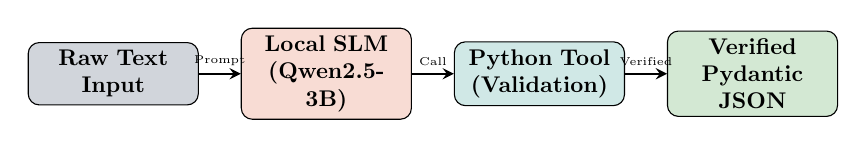
\begin{tikzpicture}[auto, >=stealth, scale=0.82, every node/.style={transform shape}]
        \node [draw, rectangle, fill=ShoePrimary!20, rounded corners, text width=2.4cm, align=center] (input) {\textbf{Raw Text Input}};
        \node [draw, rectangle, fill=ShoeAccent!20, rounded corners, text width=2.4cm, align=center, right of=input, xshift=2.3cm] (llm) {\textbf{Local SLM\\(Qwen2.5-3B)}};
        \node [draw, rectangle, fill=ShoeTeal!20, rounded corners, text width=2.4cm, align=center, right of=llm, xshift=2.3cm] (tool) {\textbf{Python Tool\\(Validation)}};
        \node [draw, rectangle, fill=ShoeGreen!20, rounded corners, text width=2.4cm, align=center, right of=tool, xshift=2.3cm] (output) {\textbf{Verified Pydantic JSON}};

        \draw [->, thick] (input) -- node[above] {\tiny Prompt} (llm);
        \draw [->, thick] (llm) -- node[above] {\tiny Call} (tool);
        \draw [->, thick] (tool) -- node[above] {\tiny Verified} (output);
    \end{tikzpicture}
    \end{center}
    \vspace{0.2cm}
    \begin{itemize}
        \item \textbf{Total Model Footprint}: 2.0 GB VRAM.
        \item \textbf{Inference Time}: 450 ms.
        \item \textbf{Cost}: \$0.000000.
    \end{itemize}
\end{frame}

% ----------------------------------------------------
% SLIDE 16: Demo Code
% ----------------------------------------------------
\begin{frame}[fragile]{Demo Walkthrough: Complete Python Implementation}
\begin{lstlisting}[language=Python,basicstyle=\ttfamily\scriptsize]
import json, ollama
from pydantic import BaseModel, Field

class ExpenseReceipt(BaseModel):
    vendor: str = Field(description="Vendor name")
    amount: float = Field(description="Total pre-tax")
    category: str = Field(description="Category (Meals, Software, Hardware)")

raw_receipt = "Cafe Java. 2 Flat Whites $9.50, 1 Muffin $4.50. Total $14.00 on 12/04."

# Ask local model with strict schema enforcement
response = ollama.chat(
    model="qwen2.5:3b",
    messages=[
        {"role": "system", "content": "Extract expense data from the receipt."},
        {"role": "user", "content": raw_receipt}
    ],
    format=ExpenseReceipt.model_json_schema()
)

data = ExpenseReceipt.model_validate_json(response['message']['content'])
print(f"Verified: {data.vendor} -> ${data.amount} ({data.category})")
# Output: Verified: Cafe Java -> $14.0 (Meals)
\end{lstlisting}
\end{frame}

% ----------------------------------------------------
% SLIDE 17: Local Coding & Test Harness
% ----------------------------------------------------
\begin{frame}{Local Coding Assistants \& Test Harnesses}
    \begin{columns}[T]
        \begin{column}{0.5\textwidth}
            \textbf{Ditching GitHub Copilot (\$10/mo):}
            \begin{itemize}
                \item \textbf{Continue.dev}: Open-source extension for VS Code / JetBrains.
                \item Connects directly to local Ollama (\texttt{qwen2.5-coder:7b}).
                \item Autocomplete (tab completion) runs on tiny 1.5B model ($\sim$20ms latency!).
                \item Chat \& refactoring runs on 7B model.
                \item \textbf{Aider}: Terminal-based pair programmer that writes git commits directly from local model edits.
            \end{itemize}
        \end{column}
        \begin{column}{0.48\textwidth}
            \begin{tcolorbox}[colback=ShoeTeal!10, colframe=ShoeTeal, title=\textbf{The Local Test Harness}]
                \small
                \textbf{How do you trust a local model?}
                \begin{itemize}
                    \item Build an automated \texttt{pytest} evaluation suite:
                    \begin{enumerate}
                        \item Feed 50 synthetic test prompts.
                        \item Assert schema validity and correct logic.
                        \item Measure latency and tokens/sec.
                    \end{enumerate}
                    \item Quantify regression before swapping model versions!
                \end{itemize}
            \end{tcolorbox}
        \end{column}
    \end{columns}
\end{frame}

% ----------------------------------------------------
% SLIDE 18: Building Custom Applications
% ----------------------------------------------------
\begin{frame}[fragile]{Building Custom Local Apps: The Shoestring Stack}
    \begin{center}
    \textbf{The Full Offline Stack: FastAPI + Gradio / Streamlit + Ollama}
    \end{center}
\begin{lstlisting}[language=Python]
from fastapi import FastAPI
import ollama

app = FastAPI(title="Shoestring Assistant API")

@app.post("/summarize")
def summarize(text: str):
    res = ollama.generate(
        model="llama3.2:3b",
        prompt=f"Summarize in 3 bullet points:\n\n{text}"
    )
    return {"summary": res['response']}
\end{lstlisting}
    \vspace{0.1cm}
    \begin{itemize}
        \item Wrap with \textbf{Streamlit} or \textbf{Gradio} for an instant web UI.
        \item Package into a single executable or self-contained Docker container.
        \item Deploy on an air-gapped office server, hospital clinic, or remote research vessel!
    \end{itemize}
\end{frame}

% ----------------------------------------------------
% SLIDE 19: AI for Personal Productivity
% ----------------------------------------------------
\begin{frame}[fragile]{Personal Productivity Hacks with Local AI}
    \begin{columns}[T]
        \begin{column}{0.48\textwidth}
            \textbf{Daily Driver Shoestring Tricks:}
            \begin{itemize}
                \item \textbf{Git Commit Generator}: Pipe \texttt{git diff} to a local model to draft conventional commit messages.
                \item \textbf{Shell Command Translator}: Forget \texttt{tar} and \texttt{find} syntax forever.
                \item \textbf{Local Meeting Transcripts}: Run \texttt{whisper.cpp} locally for audio-to-text, then pass to \texttt{llama3.2} for bullet summaries.
                \item \textbf{Markdown Notes Search}: Semantic query across thousands of Obsidian or Notion export notes.
            \end{itemize}
        \end{column}
        \begin{column}{0.48\textwidth}
            \begin{block}{\textbf{One-Liner Bash Aliases}}
\begin{lstlisting}[language=bash]
# Add to ~/.bashrc or ~/.zshrc:
alias q="ollama run qwen2.5:3b"

# Commit generator alias:
function aicommit() {
  git diff --staged | ollama run \
    qwen2.5-coder:3b \
    "Write a concise git commit message for this diff:" \
    | git commit -F -
}
\end{lstlisting}
            \end{block}
            \centering
            \alert{No telemetry. No rate limits. Instant response.}
        \end{column}
    \end{columns}
\end{frame}

% ----------------------------------------------------
% SLIDE 20: Hardware Sizing Guide
% ----------------------------------------------------
\begin{frame}{Hardware Sizing Guide: What Can Your Rig Run?}
    \begin{table}
        \small
        \begin{tabular}{llll}
            \toprule
            \textbf{Your Hardware Tier} & \textbf{Max Model Size} & \textbf{Recommended Model} & \textbf{Tokens/sec} \\
            \midrule
            \textbf{Potato PC} (8GB RAM, CPU only) & 1B -- 3B (Q4) & Llama-3.2-1B, SmolLM2 & 15--25 t/s \\
            \textbf{Everyday Laptop} (16GB RAM) & 7B -- 8B (Q4) & Qwen2.5-7B, Llama-3.1-8B & 8--14 t/s \\
            \textbf{Gaming PC} (8GB VRAM RTX 3060) & 8B (Q4 offloaded) & Llama-3.1-8B-Instruct & 45--65 t/s \\
            \textbf{Apple Silicon} (36GB--64GB M-series) & 32B -- 70B (Q4) & Qwen2.5-32B, Llama-70B & 12--25 t/s \\
            \textbf{Colibr\`i Mode} (24GB RAM + NVMe) & \textbf{744B MoE} (Q4) & GLM-4/5.2 MoE & $\sim$1 t/s \\
            \bottomrule
        \end{tabular}
    \end{table}
    \vspace{0.3cm}
    \begin{tcolorbox}[colback=ShoeAccent!10, colframe=ShoeAccent, title=\textbf{The Golden Memory Rule}]
        \small
        \textbf{Always leave 3--4 GB RAM for your operating system}, or your browser and Spotify will wage war against your model!
    \end{tcolorbox}
\end{frame}

% ----------------------------------------------------
% SLIDE 21: Common Pitfalls & Traps
% ----------------------------------------------------
\begin{frame}{Common Traps \& Anti-Patterns}
    \begin{columns}[T]
        \begin{column}{0.48\textwidth}
            \begin{alertblock}{\textbf{What NOT To Do}}
                \begin{itemize}
                    \item \textbf{Downloading FP16}: Wondering why your 7B model took 16GB and crashed your machine.
                    \item \textbf{Context Window Bloat}: Setting context to 128k tokens on an 8GB machine eats all RAM just for the KV-cache!
                    \item \textbf{Ignoring Quant Types}: Downloading \texttt{Q2\_K} just because it's tiny, then complaining the model thinks $2+2=5$.
                    \item \textbf{Running without GPU Offload}: Forgetting to check if your CUDA / Metal backend is active.
                \end{itemize}
            \end{alertblock}
        \end{column}
        \begin{column}{0.48\textwidth}
            \begin{exampleblock}{\textbf{The Shoestring Best Practices}}
                \begin{itemize}
                    \item \textbf{Stick to Q4\_K\_M or Q5\_K\_M} for general tasks.
                    \item \textbf{Tune Context Appropriately}: Set context window to 4k or 8k unless you really need to ingest an entire book.
                    \item \textbf{Use KV-Cache Quantization}: \texttt{llama.cpp} flag \texttt{--cache-type-k q8\_0} slashes context RAM in half!
                    \item \textbf{Embrace MoE architectures} (like Colibr\`i) for high capability with reduced memory footprint.
                \end{itemize}
            \end{exampleblock}
        \end{column}
    \end{columns}
\end{frame}

% ----------------------------------------------------
% SLIDE 22: Summary & Conclusion
% ----------------------------------------------------
\begin{frame}{Summary: The Democratization of Intelligence}
    \begin{itemize}
        \item[\checkmark] \textbf{Independence}: You do not need billions in venture capital or corporate API keys to harness cutting-edge AI.
        \item[\checkmark] \textbf{The Stack}: Ollama + GGUF + Python OpenAI client + ChromaDB gives you an enterprise-grade agent and RAG platform.
        \item[\checkmark] \textbf{Extreme Engineering}: The \textbf{Colibr\`i Project} proves that architectural ingenuity (MoE + NVMe streaming in pure C) punches through hardware limits.
        \item[\checkmark] \textbf{Speed \& Security}: Zero latency variability, total confidentiality, infinite experimentation at zero marginal cost.
    \end{itemize}
    \vspace{0.4cm}
    \begin{tcolorbox}[colback=ShoeTeal!10, colframe=ShoeTeal, title=\textbf{Final Thought}]
        \large\centering
        \textbf{The future of AI is not in a distant cloud datacenter.\\It is right here, compiled on your laptop.}
    \end{tcolorbox}
\end{frame}

% ----------------------------------------------------
% SLIDE 23: Q&A and Resources
% ----------------------------------------------------
\begin{frame}{Resources \& Shoestring Toolkit}
    \begin{columns}[T]
        \begin{column}{0.5\textwidth}
            \textbf{Essential Repositories:}
            \begin{itemize}
                \item \textbf{Ollama}: \url{https://ollama.com}
                \item \textbf{llama.cpp}: \url{https://github.com/ggerganov/llama.cpp}
                \item \textbf{Colibr\`i Project}: Pure C MoE NVMe streaming inference engine
                \item \textbf{LM Studio}: \url{https://lmstudio.ai}
                \item \textbf{Continue.dev}: Open source IDE copilot
                \item \textbf{ChromaDB}: Serverless local vector DB
            \end{itemize}
        \end{column}
        \begin{column}{0.48\textwidth}
            \begin{tcolorbox}[colback=ShoePrimary!10, colframe=ShoePrimary, title=\textbf{Now Go Build!}]
                \small
                \begin{itemize}
                    \item Grab an 8B model.
                    \item Quantize to Q4.
                    \item Write a local agent loop.
                    \item Keep your data, keep your money.
                \end{itemize}
                \vspace{0.2cm}
                \textbf{Questions \& Answers}
            \end{tcolorbox}
        \end{column}
    \end{columns}
\end{frame}

\end{document}
